\documentclass[a4paper,twoside,11pt]{article}
\usepackage{a4wide,graphicx,fancyhdr,amsmath,amssymb}
\usepackage{listings}
\usepackage{color}
\usepackage{enumitem}
\usepackage{amsmath}

%----------------------- Macros and Definitions --------------------------

\setlength\headheight{20pt}
\addtolength\topmargin{-10pt}
\addtolength\footskip{20pt}

\newcommand{\N}{\mathbb{N}}
\newcommand{\ch}{\mathcal{CH}}

\newcommand{\solution}[1]{\noindent{\bf Solution to Exercise #1:}}

\fancypagestyle{plain}{%
\fancyhf{}
\fancyhead[LO,RE]{\sffamily\bfseries\large technische universiteit eindhoven}
\fancyhead[RO,LE]{\sffamily\bfseries\large 2IW02 RTSD}
\fancyfoot[LO,RE]{\sffamily\bfseries\large department of mathematics and computer science}
\fancyfoot[RO,LE]{\sffamily\bfseries\thepage}
\renewcommand{\headrulewidth}{0pt}
\renewcommand{\footrulewidth}{0pt}
}

\pagestyle{fancy}
\fancyhf{}
\fancyhead[RO,LE]{\sffamily\bfseries\large technische universiteit eindhoven}
\fancyhead[LO,RE]{\sffamily\bfseries\large 2IW02 RTSD}
\fancyfoot[LO,RE]{\sffamily\bfseries\large department of mathematics and computer science}
\fancyfoot[RO,LE]{\sffamily\bfseries\thepage}
\renewcommand{\headrulewidth}{1pt}
\renewcommand{\footrulewidth}{0pt}

%-------------------------------- Title ----------------------------------

\title{\vspace{-\baselineskip}\sffamily\bfseries Exercise 1}
\author{
	Rick Veens \qquad Studentno: 0912292\\
	\texttt{r.veens@student.tue.nl}
	\and
	Huib Donkers \qquad Studentno: 0769015\\
	\texttt{h.t.donkers@student.tue.nl}
}

\date{\today}

\definecolor{listinggray}{gray}{0.9}
\definecolor{lbcolor}{rgb}{0.9,0.9,0.9}
\lstset{
backgroundcolor=\color{lbcolor},
    tabsize=4,    
%   rulecolor=,
    language=[GNU]C++,
        basicstyle=\scriptsize,
        upquote=true,
        aboveskip={1.5\baselineskip},
        columns=fixed,
        showstringspaces=false,
        extendedchars=false,
        breaklines=true,
        prebreak = \raisebox{0ex}[0ex][0ex]{\ensuremath{\hookleftarrow}},
        frame=single,
        numbers=left,
        showtabs=false,
        showspaces=false,
        showstringspaces=false,
        identifierstyle=\ttfamily,
        keywordstyle=\color[rgb]{0,0,1},
        commentstyle=\color[rgb]{0.026,0.112,0.095},
        stringstyle=\color[rgb]{0.627,0.126,0.941},
        numberstyle=\color[rgb]{0.205, 0.142, 0.73},
%        \lstdefinestyle{C++}{language=C++,style=numbers}’.
}

% geen stomme indents bij \par
\setlength{\parindent}{0cm}

%--------------------------------- Text ----------------------------------

\begin{document}
\maketitle

\section{}
\subsection{}
\subsubsection{}
SystemDF:\\
	\centerline{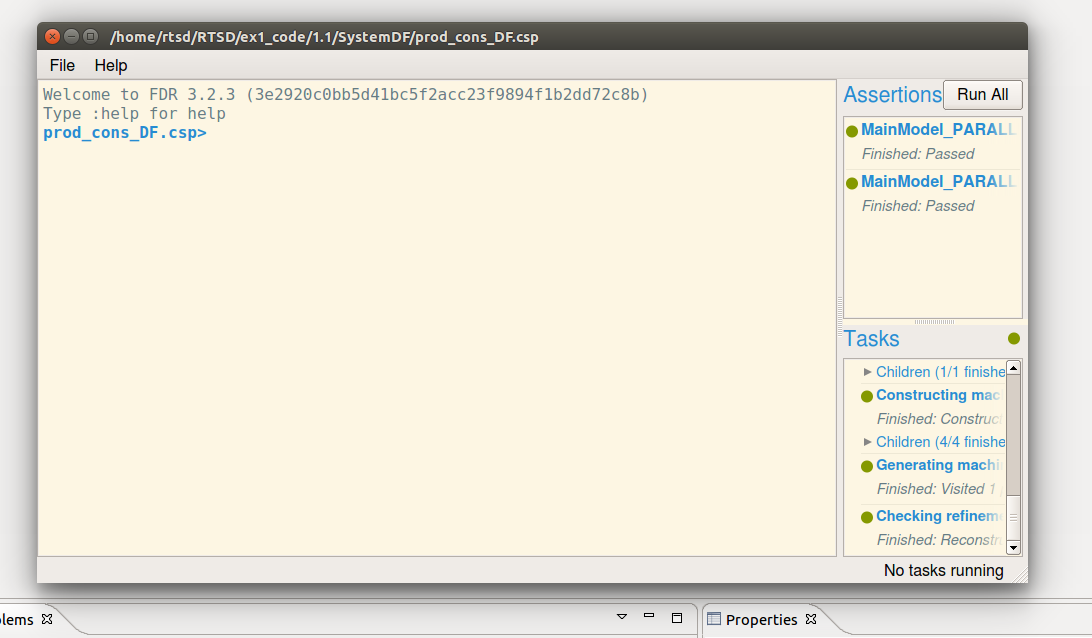
\includegraphics[width=\linewidth]{./images/1_1-SystemDF.png}}
	\centerline{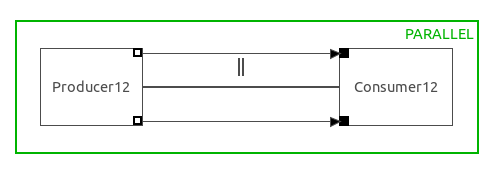
\includegraphics[width=\linewidth]{./images/1_1-SystemDF_main.png}}
	\centerline{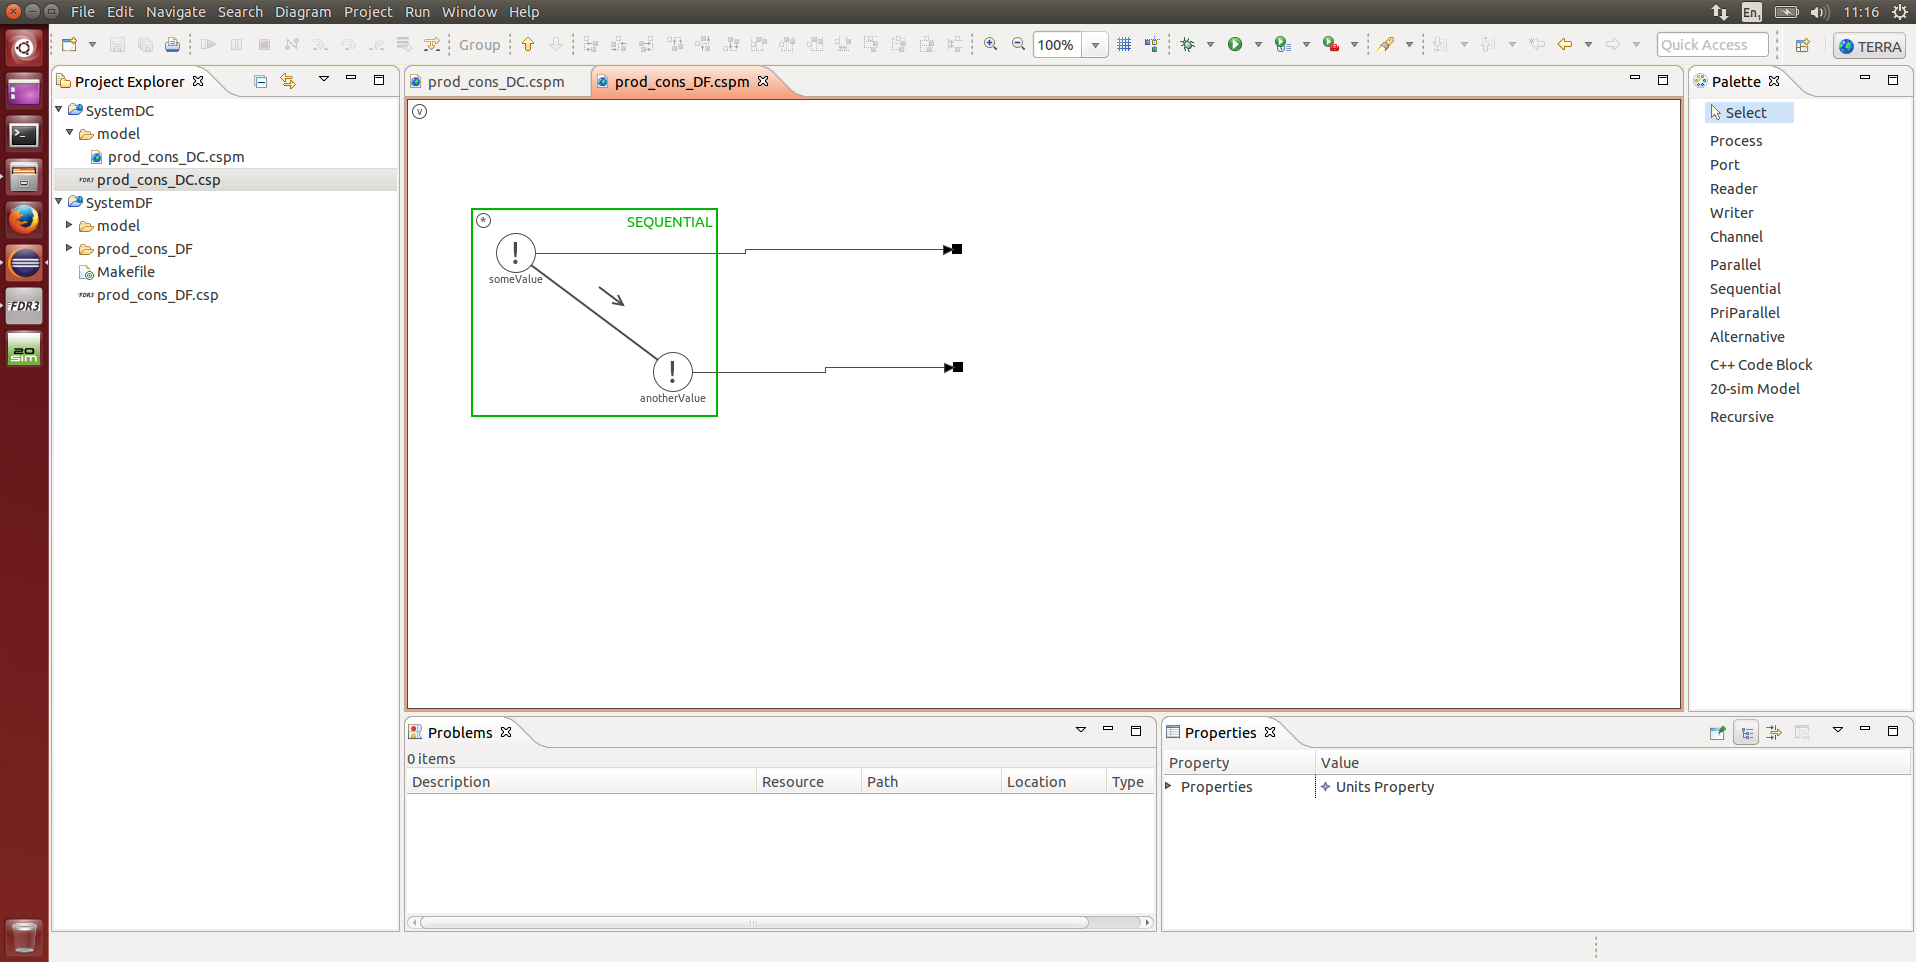
\includegraphics[width=\linewidth]{./images/1_1-SystemDF_cons.png}}
	\centerline{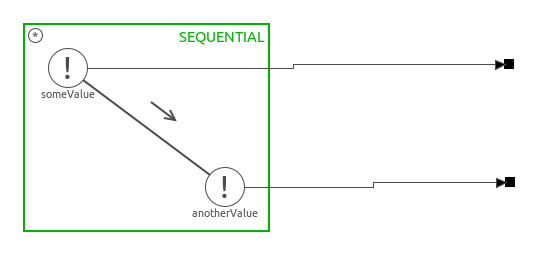
\includegraphics[width=\linewidth]{./images/1_1-SystemDF_prod.png}}

SystemDC:\\
	\centerline{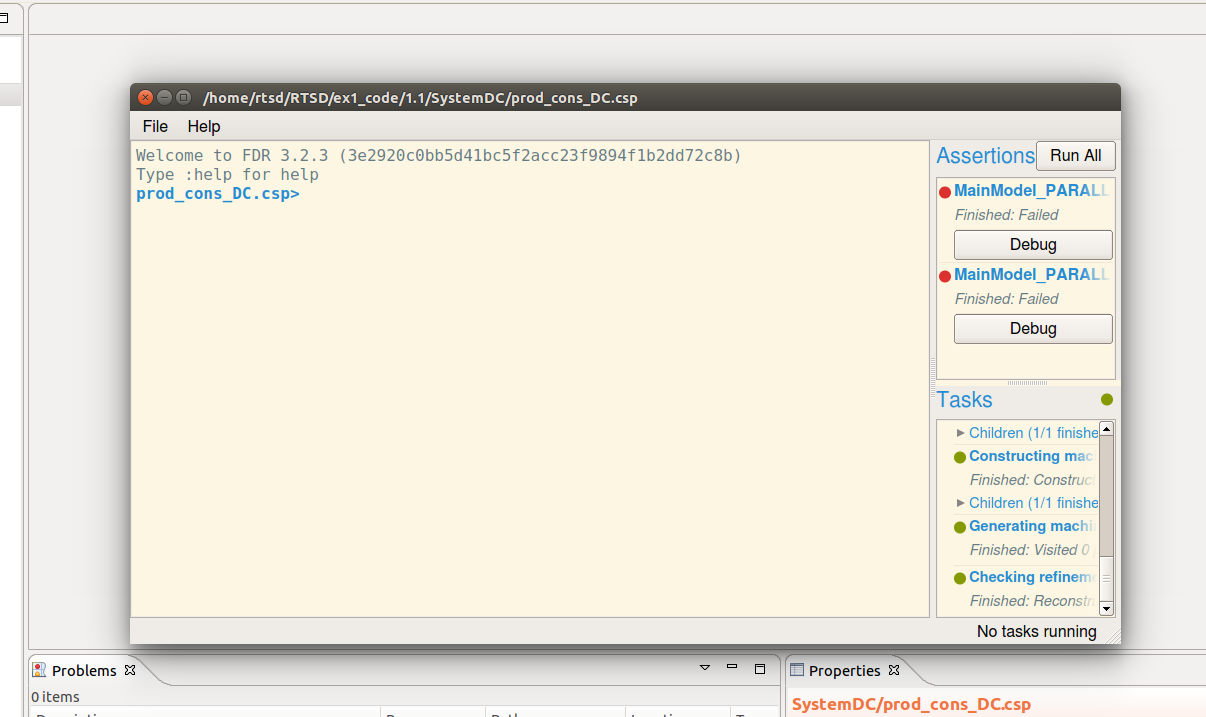
\includegraphics[width=\linewidth]{./images/1_1-SystemDC.png}}
	\centerline{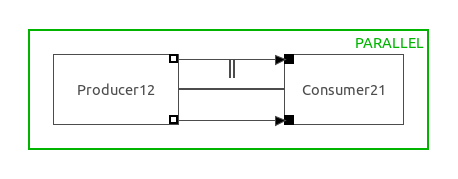
\includegraphics[width=\linewidth]{./images/1_1-SystemDC_main.png}}
	\centerline{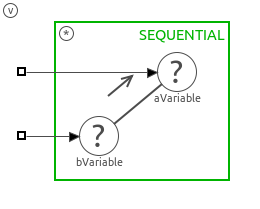
\includegraphics[width=\linewidth]{./images/1_1-SystemDC_cons.png}}
	\centerline{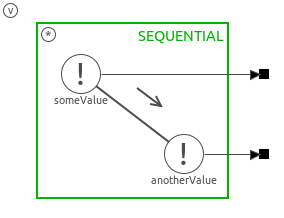
\includegraphics[width=\linewidth]{./images/1_1-SystemDC_prod.png}}

\subsubsection{}
Consumer:\\
	\centerline{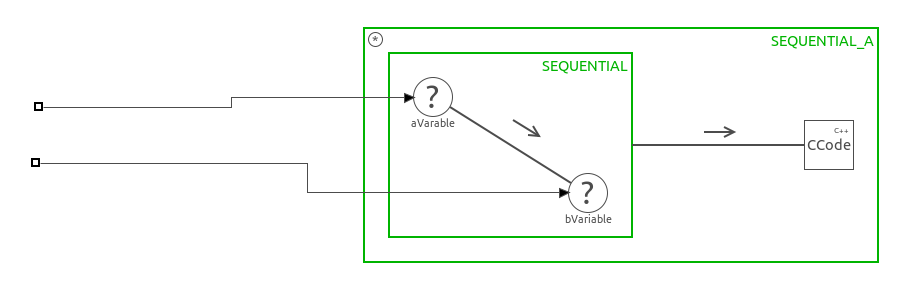
\includegraphics[width=\linewidth]{./images/1_2-SystemDF+_cons.png}}

Producer:\\
	\centerline{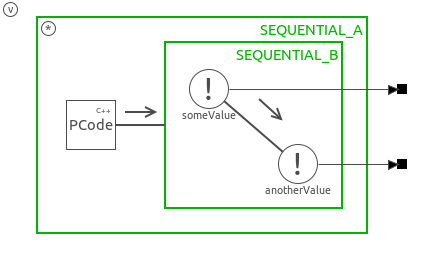
\includegraphics[width=\linewidth]{./images/1_2-SystemDF+_prod.png}}

Code:

Consumer12/CCode.cpp:
\begin{lstlisting}[language=C++]
/**
 * Source file for the CCode model
 * Generated by the TERRA CSPm2LUNA generator version 1.1.1
 *
 * protected region document description on begin
 *
 * protected region document description end
 */

#include "Consumer12/CCode.h"
// protected region additional headers on begin
// Each additional header should get a corresponding dependency in the Makefile
// protected region additional headers end

namespace MainModel { namespace Consumer12 { namespace CCode { 

CCode::CCode(int &CCode_aVariable, int &CCode_bVariable) :
    CodeBlock(), CCode_aVariable(CCode_aVariable), CCode_bVariable(CCode_bVariable){
  SETNAME(this, "CCode");

  // protected region constructor on begin
  // protected region constructor end
}

CCode::~CCode()
{
  // protected region destructor on begin
  // protected region destructor end
}

void CCode::execute()
{
  // protected region execute code on begin
	if (this->CCode_aVariable == -1 || this->CCode_bVariable == -1)
		exit();
	else {
		printf("Receiving: CCode_aVariable: \t'%c'\n", this->CCode_aVariable);
		printf("Receiving: CCode_bVariable: \t'%c'\n", this->CCode_bVariable);

		printf("\n");
	}
  // protected region execute code end
}

// protected region additional functions on begin
// protected region additional functions end

// Close namespace(s)
} } } 
\end{lstlisting}

Producer12/PCode.cpp:
\begin{lstlisting}[language=C++]
/**
 * Source file for the PCode model
 * Generated by the TERRA CSPm2LUNA generator version 1.1.1
 *
 * protected region document description on begin
 *
 * protected region document description end
 */

#include "Producer12/PCode.h"
#include "string.h"
// protected region additional headers on begin
// Each additional header should get a corresponding dependency in the Makefile
// protected region additional headers end

namespace MainModel { namespace Producer12 { namespace PCode { 

PCode::PCode(int &PCode_anotherValue, int &PCode_someValue) :
    CodeBlock(), PCode_anotherValue(PCode_anotherValue), PCode_someValue(PCode_someValue){
  SETNAME(this, "PCode");

  // protected region constructor on begin
  // protected region constructor end
}

PCode::~PCode()
{
  // protected region destructor on begin
  // protected region destructor end
}

void PCode::execute()
{
  // protected region execute code on begin

	static int index = 0;

	char *stuff = "Appelflap";

	if (index == strlen(stuff)) {
		this->PCode_someValue = -1;
		this->PCode_anotherValue = -1;
	} else {
		this->PCode_someValue = stuff[index];
		this->PCode_anotherValue = stuff[index++];

		printf("Sending: PCode_someValue: \t'%c'\n", this->PCode_someValue);
		printf("Sending: PCode_anotherValue: \t'%c'\n", this->PCode_anotherValue);
	}


  // protected region execute code end
}

// protected region additional functions on begin
// protected region additional functions end

// Close namespace(s)
} } } 
\end{lstlisting}

Output:\\
	\centerline{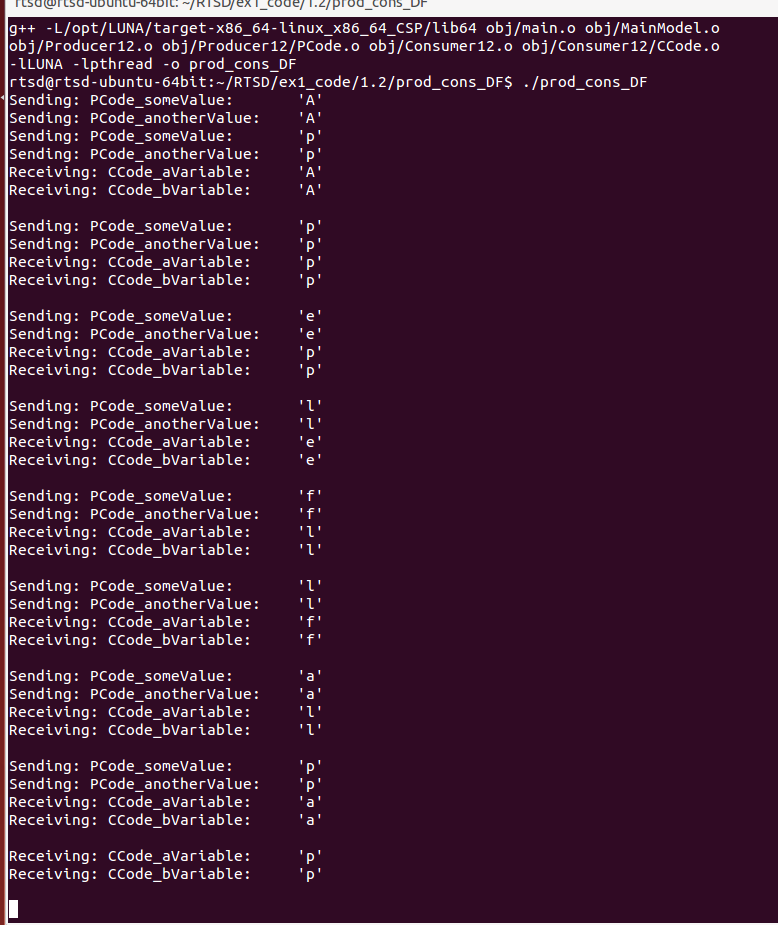
\includegraphics[width=\linewidth]{./images/1_2-SystemDF+_output.png}}

\subsubsection{}
Sometimes value B gets send before value A is received.
However, the values are still received in the correct order.

It appears to be that, the communication between the writers and readers are synchronized, but not the code that we added for printing sent and receive values.

So it might occur that the printing-code of the next value B, is executed before the printing-code of the received value A.
\subsubsection{}
\color{red}
ProBE is used to view the traces of processes only. FDR can be used to check for deadlocks and livelocks.
\color{black}

\subsubsection{}
test

\end{document}
